\section{Editare draft}

Operațiunile permise asupra unui draft sunt modelate la nivelul domeniului prin interfața \texttt{DraftsUseCase}, după cum este prezentată în programul \ref{lst:draftsUseCase}. Atât funcționalitatea de listare, cât și cea de editare se folosesc de funcționalitatea \emph{Room} prin care atunci când apare o modificare la nivelul bazei de date, o nouă valoare este emisă pentru interogările deja executate. Astfel, este ușoară o implementare reactivă pentru acestea.

\lstinputlisting[style=javaCodeStyle, caption={Interfața Drafts Use Case}, label={lst:draftsUseCase}]{./code/DraftsUseCase.kt}

Editarea câmpurilor text se face în manieră \emph{on the fly}, ceea ce înseamnă că nu este necesar un ecran separat drept formular și apăsarea unui buton de persistare a modificărilor. La nivelul interfeței grafice, câmpurile textuale sunt reprezentate prin câmpuri \texttt{EditText}, care permit tastarea în interior. De fiecare dată când utilizatorul face modificări asupra acestor câmpuri, o funcție \emph{callback} este declanșată, care apelează funcția de actualizare valorii în baza de date.

Pentru ca actualizarea să nu se producă mult prea des, funcțiilor de actualizare le este aplicat operatorul \texttt{throttleLast}. Funcționarea acestuia este ilustrată în figura \ref{fig:throttle}\cite{ThrottleLast}. Acest operator emite obiecte numai după ce un anumit timp a trecut. Aplicarea acestui operator unei funcții se face prin crearea unui obiect \texttt{PublishSubject} și este ilustrată în programul \ref{lst:throttle}.

\lstinputlisting[style=javaCodeStyle, caption=Funcții throttled,label=lst:throttle]{./code/ThrottleImplementation.kt}

\begin{figure}[ht]
  \centering
  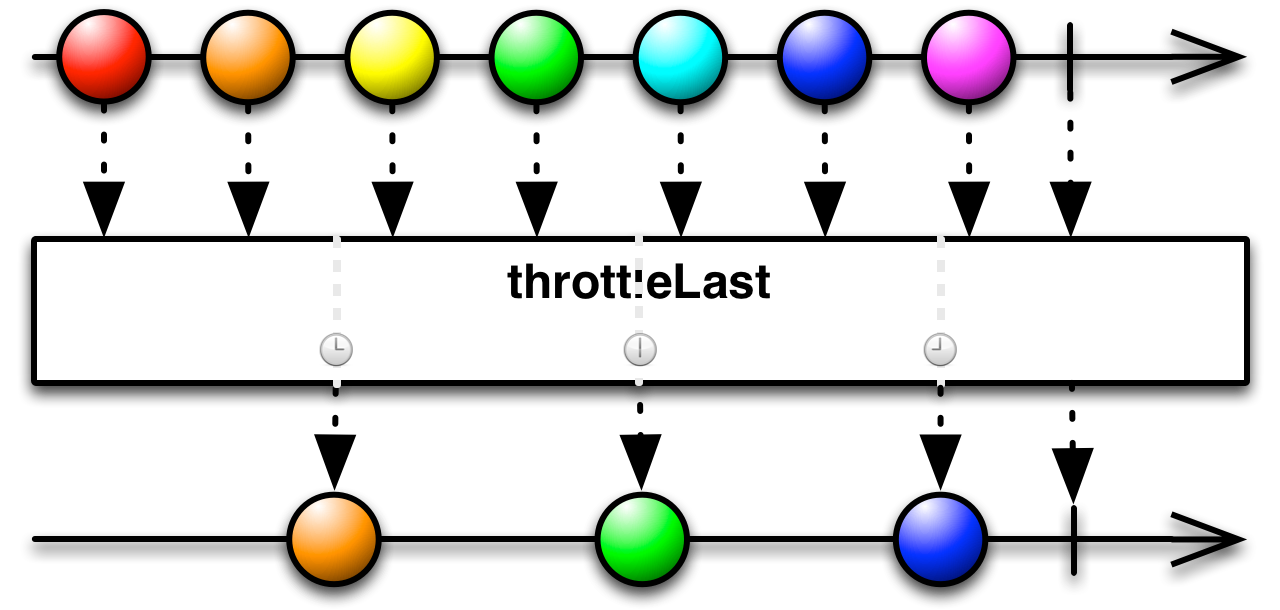
\includegraphics[width=0.7\textwidth]{throttleLast.png}
  \caption{Operatorul throttleLast}
  \label{fig:throttle}
\end{figure}

Baza de date este actualizată cu valori compuse de tipul \texttt{Draft}. De aceea funcția \texttt{update} primește o nouă valoare singulară și o funcție care are ca argumente noua valoare unitară și vechea valoare \texttt{Draft} și emite valoarea compusă nouă, ce este persistată. Implementarea acestei funcții se face folosind funcția \texttt{copy} ce este definită automat pentru clase de date în \emph{Kotlin}.

Obiectul vizual din \emph{Android} predefinit pentru afișarea imaginilor  nu permite gestul de \emph{zoom}. Pentru a oferi această funcționalitate pentru imaginea draftului curent, am folosit librăria \emph{PhotoView} \cite{PhotoView}. 
